\documentclass[11pt]{article}
\usepackage{amsmath,amsthm,amssymb}
\usepackage{tikz,tikz-network}
\usetikzlibrary{arrows}

\begin{document}

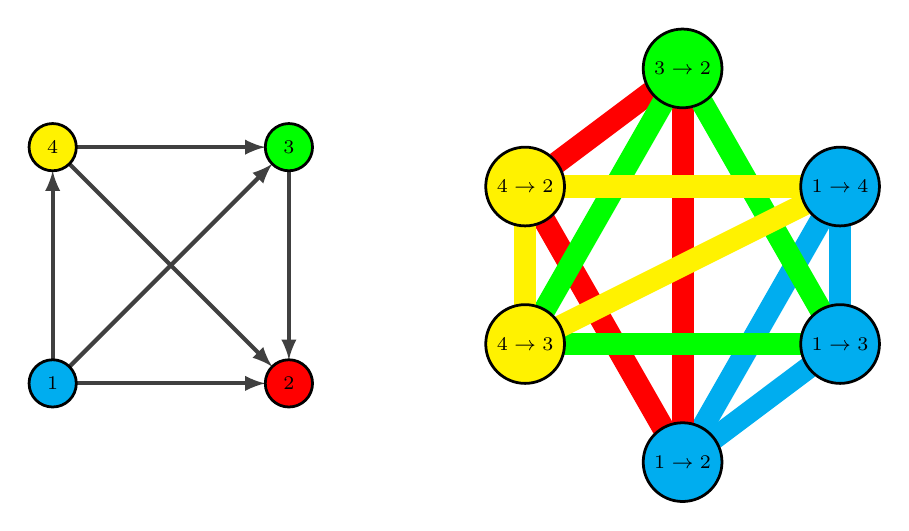
\begin{tikzpicture}
	\Vertex[color=cyan,label=1]{A}
	\Vertex[color=red,x=3,label=2]{B}
	\Vertex[color=green,x=3,y=3, label=3]{C}
	\Vertex[color=yellow,y=3, label=4]{D}
	\Edge[Direct](A)(B)
	\Edge[Direct](A)(C)
	\Edge[Direct](A)(D)
	\Edge[Direct](C)(B)
	\Edge[Direct](D)(C)
	\Edge[Direct](D)(B)
	\Vertex[x=8,y=-1,size=1,label=1\to 2,Math,color=cyan]{E}
	\Vertex[x=10,y=0.5,size=1,label=1\to 3,Math,color=cyan]{F}
	\Vertex[x=10,y=2.5,size=1,label=1\to 4,Math,color=cyan]{G}
	\Vertex[x=8,y=4,size=1,label=3\to 2,Math,color=green]{H}
	\Vertex[x=6,y=2.5,size=1,label=4\to 2,Math,color=yellow]{I}
	\Vertex[x=6,y=0.5,size=1,label=4\to 3,Math,color=yellow]{J}
	\Edge[lw=8pt,color=cyan](E)(F)
	\Edge[lw=8pt,color=cyan](E)(G)
	\Edge[lw=8pt,color=cyan](G)(F)
	\Edge[lw=8pt,color=red](E)(H)
	\Edge[lw=8pt,color=red](H)(I)
	\Edge[lw=8pt,color=red](E)(I)
	\Edge[lw=8pt,color=green](J)(F)
	\Edge[lw=8pt,color=green](H)(F)
	\Edge[lw=8pt,color=green](H)(J)
	\Edge[lw=8pt,color=yellow](I)(J)
	\Edge[lw=8pt,color=yellow](G)(I)
	\Edge[lw=8pt,color=yellow](G)(J)
\end{tikzpicture}

\end{document}